
\chapter{Aplicacion en un modelo fisico de laboratorio}

\section{Descripcion del modelo}

Los ensayos que se llevaron a cabo en este trabajo se realizaron en un modelo fisico ubicado en el Laboratorio de Hidraulica [CITAR] de la Facultad de Ciencias Exactas, Fisicas y Naturales (UNC). El modelo es una representacion a escala reducida 1:65 del Dique Los Molinos, ubicado en la provincia Jujuy.

% ELEGIR OTRA IMAGEN POR QUE EN ESTA EL MODELO ESTA EN CONSTRUCCION
\begin{figure}[ht]
\centering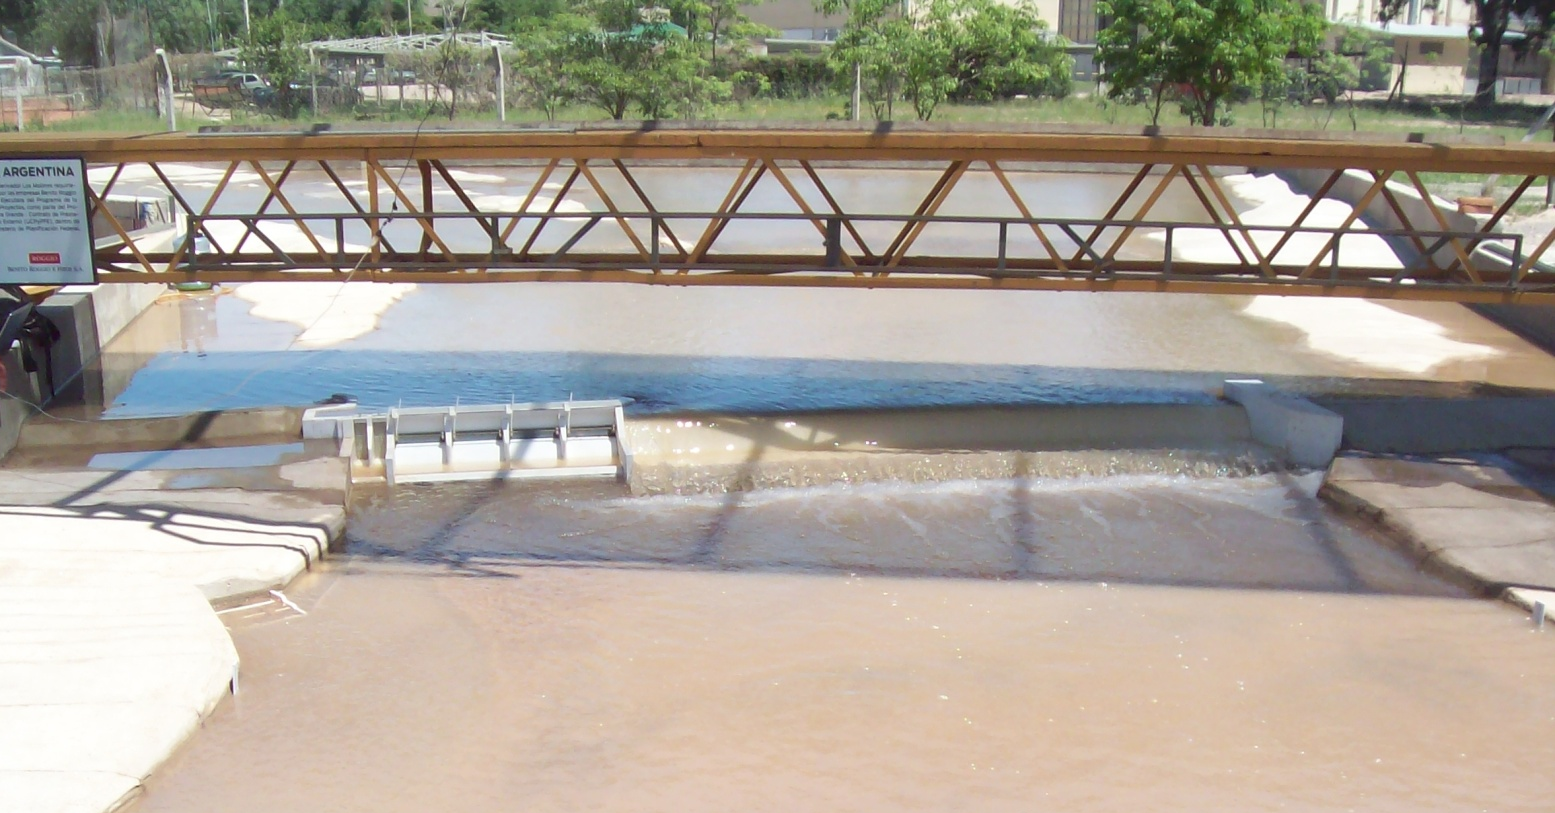
\includegraphics[width=\imsizeS]
{modelo-fisico-dique-los-molinos}
\caption[Modelo fisico dique Los Molinos]{Modelo fisico dique Los Molinos, Laboratorio de Hidráulica, FCEFyN de la UNC.}
\label{fig:modelo-fisico-dique-los-molinos}
\end{figure}

% ELEGIR OTRA IMAGEN SIN EXPLICACION DE LAS COMPONENTES
\begin{figure}[ht]
\centering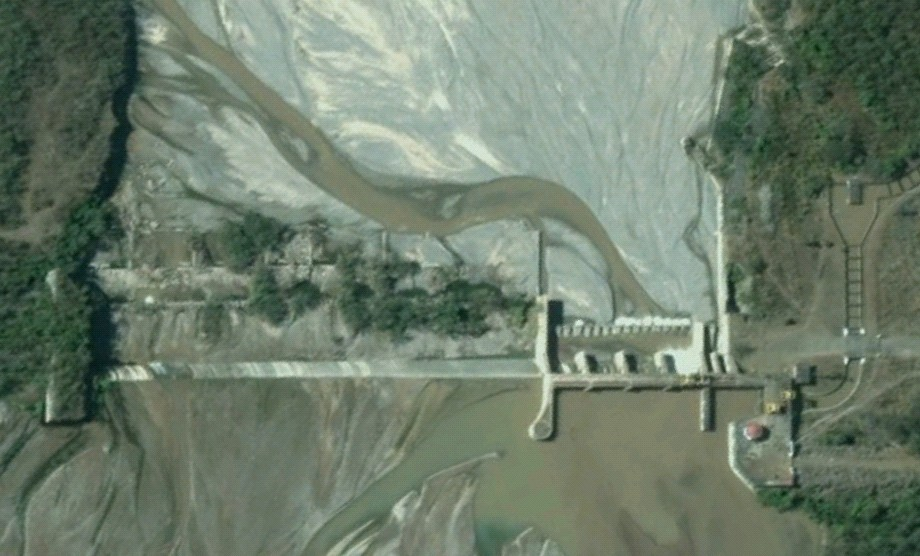
\includegraphics[width=\imsizeS]
{dique-los-molinos}
\caption[Dique Los Molinos]{Dique Los Molinos, Jujuy.}
\label{fig:dique-los-molinos}
\end{figure}

Sobre la zona de interes, se ha construido una plataforma movil que posibilita realizar las mediciones de erosion. La plataforma esta compuesta por : 

\begin{itemize}

\item Un puente grua. Este puede ser trasladado para observar distintas areas del modelo.

\item Una guia-riel y un carro-soporte para la camara Kinect. Ver \ref{fig:sistema-camara-carro}. La guia se anexa al puente grua, lo que permite la translacion de la camara a lo ancho del modelo. AGREGAR SOBRE LA EXTENSION.

\end{itemize}

\begin{figure}[ht]
\centering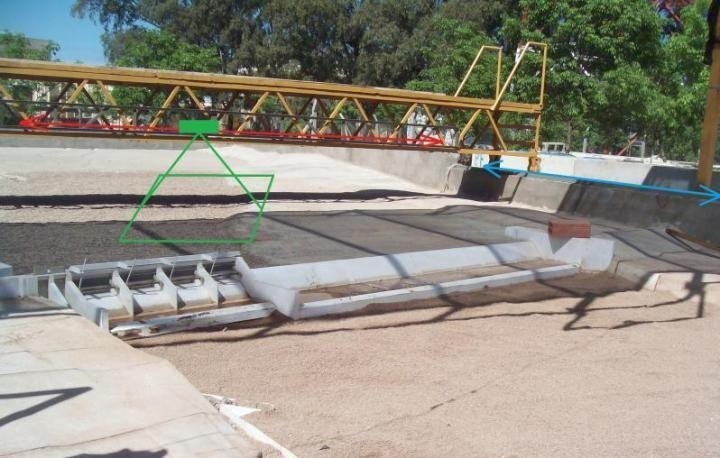
\includegraphics[width=\imsize]
{esquema-camara-puente-grua}
\caption[Puente grua]{Puente grua. Las flechas representan la direccion del movimiento de la camara (esquematizada con el recuadro verde). En rojo, sobre el puente grua y en azul el movimiento del puente grua sobre el modelo.}
\label{fig:esquema-camara-puente-grua}
\end{figure}

\begin{figure}[ht]
\centering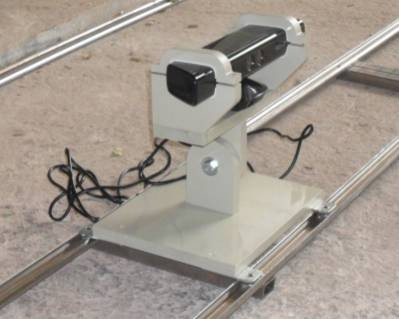
\includegraphics[width=\imsize]
{sistema-camara-carro}
\caption[Sistema camara-soporte]{Soporte construido para trasladar la camara sobre el modelo.}
\label{fig:sistema-camara-carro}
\end{figure}

%%%%%%%%%%%%%%%%%%%%%%%%%%%%%%%%%%%%%%%%%%%%%%%%%%%%%%%%%%%%%%%%%%%%%%%%%%%%%%%

\section{Ensayos realizados}

\subsection{Erosion maxima}

\subsection{Formas de fondo}

%%%%%%%%%%%%%%%%%%%%%%%%%%%%%%%%%%%%%%%%%%%%%%%%%%%%%%%%%%%%%%%%%%%%%%%%%%%%%%%
\section{Consideraciones generales}

Como parte de la metodologia de medicion, hay consideraciones que deben tenerse en cuenta :
\begin{itemize}

\item La superfie debe estar libre de agua. Como se menciono en \ref{sec:consideraciones-kinect}, objetos con caracteristicas reflectantes afectan al sensor de profundidad de la Kinect. Figura \ref{fig:modelo-condiciones-agua}.

\item La escena debe estar al resguardo de la luz solar, como se explica en \ref{sec:consideraciones-kinect}. Para esto se utilizo un nylon de color negro colocado sobre el puente grua, como se puede observar en las figuras \ref{fig:modelo-lona1} y \ref{fig:modelo-lona2}. Tambien se considero realizar las mediciones al atardecer cuando la luz solar es mas tenue. Se pudo observar que
utilizando el nylon se obtienen condiciones luminicas mas estables, sin importar el 
horario.

\item La guia debe estar perfectamente nivelada. Un par de centrimetros de desnivel conllevan grandes inconsistencias en las estructuras del dique cuando se convierten los datos a escala prototipo.

\item La camara debe ubicarse a una altura minima de 0.4 m y a una altura maxima de 2m [REVISAR] de la escena para que el error se mantenga dentro de un intervalo aceptable \ref{sec:consideraciones-kinect}. EXPLICAR MAS.

\end{itemize}

\begin{figure}[h]
\centering
\begin{minipage}[t]{.45\textwidth}
\begin{center}
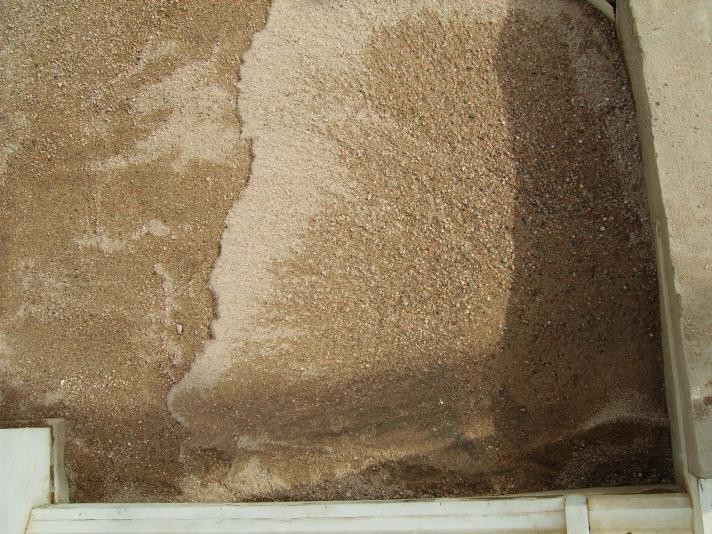
\includegraphics[width=\imsizeS]{modelo-sin-agua} % primera imagen colocada a la izquierda
\end{center}
\end{minipage}
\hfill
\begin{minipage}[t]{.45\textwidth}
\begin{center}
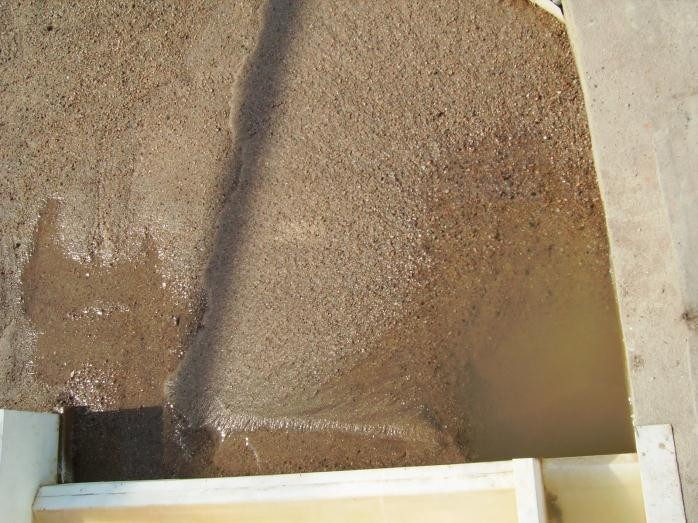
\includegraphics[width=\imsizeS]{modelo-con-agua} % segunda imagen colocada a la derecha
\end{center}
\end{minipage}
\hfill
\caption{A la derecha condicion correcta para la medicion. A la izquiera se observan espejos de agua que interfieren el sensor infrarojo de la camara.}
\label{fig:modelo-condiciones-agua}
\end{figure}



\begin{figure}[ht]
\centering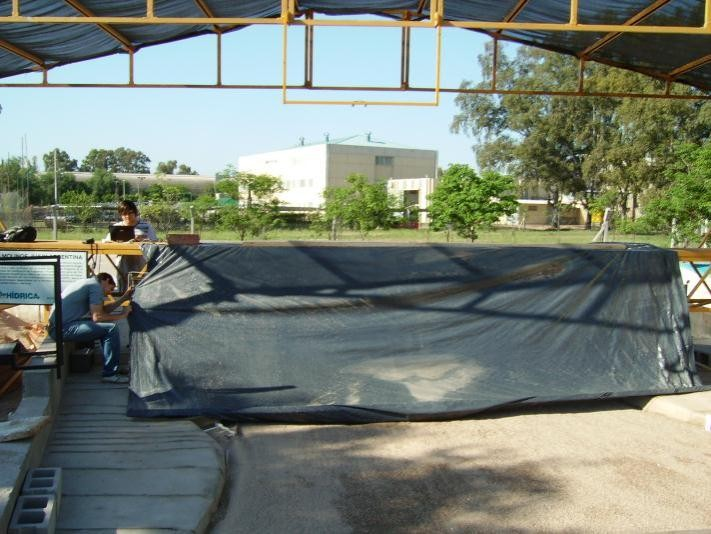
\includegraphics[width=\imsizeS]
{modelo-lona1}
\caption[Modelo cubierto por nylon.]
{Forma de colocar el nylon sobre el puente grua para cubrir todo el largo del riel.}
\label{fig:modelo-lona1}
\end{figure}

\begin{figure}[ht]
\centering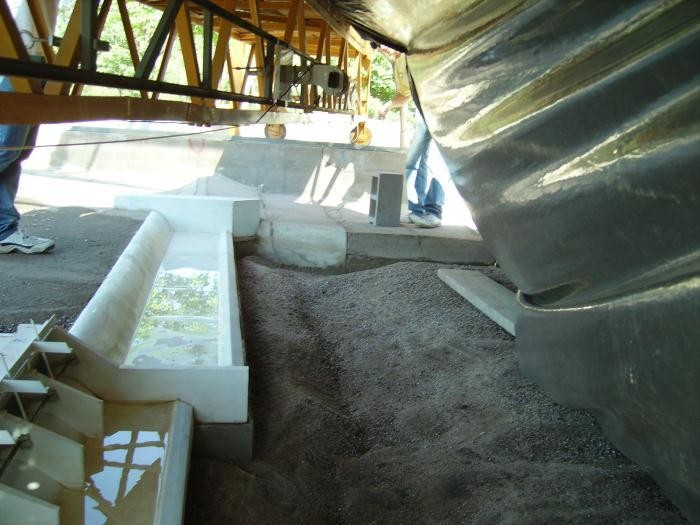
\includegraphics[width=\imsizeS]
{modelo-lona2}
\caption[Sombra generada por nylon sobre el modelo.]
{Sombra producida por el nylon para tomar imagenes sin interferencias.}
\label{fig:modelo-lona2}
\end{figure}